In Chapter \ref{ch:functors} we presented a language extension for Metacasanova that allows to drastically improve the performance of the generated code with functors. In this chapter we show how this language extension can be used to improve the performance and further extend the domain-specific language Casanova implemented in Metacasanova with language primitives for online multiplayer game development. We start this chapter by introducing the problem of developing an online multiplayer game and the existing approaches. We then propose a language extension for Casanova to integrate primitives to support network data synchronization that should aid the developer of online multiplayer games, which has also been peresented in \cite{DIGIACOMO201725}. We then proceed to show how to implement the entity update for Casanova by using functors in Metacasanova and evaluate its performance gain. We conclude the chapter by showing that functors can be used to further extend Casanova in Metacasanova with the same networking primitives that we had earlier introduced.

\section{Multi-player Support in Games}
Adding multi-player support to games is a highly desirable feature. By letting players interact with each other, new forms of gameplay, cooperation, and competition emerge without requiring any additional design of game mechanics \cite{granberg2014david}. This allows a game to remain fresh and playable, even after the single player content has been exhausted. For example, consider any modern AAA (AAA refers to games with the highest development budgets\cite{wolf2008video}) game such as \textit{Halo 4}. After months since its initial release, most players have exhausted the single player, narrative-driven campaign. Nevertheless the game remains heavily in use thanks to multiplayer modes, which in effect extended the life of the game significantly. This phenomenon is even more evident in games such as \textit{World of Warcraft} or \textit{EVE}, where multiplayer is the only modality of play and there is no single-player experience.

\paragraph{Challenges}
Multi-player support in games is a very expensive piece of software to build. Multiplayer games are under strong pressure to have very good \textit{performance} \cite{claypool2006latency}. Performance is both expressed in terms of CPU time and in bandwidth used. Also, games need to be very \textit{robust} with respect to transmission delays, packets lost, or even clients disconnected. To make matters worse, players often behave erratically. It is widespread practice among players to leave a competitive game as soon as their defeat is apparent (a phenomenon so common to even have its own name: ``rage quitting'' \cite{rage_quitting}), or to try to abuse the game and its technical flaws to gain advantages or to disrupt the experience of others.

Networking code reuse is quite low across titles and projects. This comes from the fact that the requirements of every game vary significantly: from turn-based games that only need to synchronize the game world every few seconds, and where latency is not a big issue, to first-person-shooter games where prediction mechanisms are needed to ensure the smooth movement of synchronized entities, to real-time strategy games where thousands of units on the screen all need to be synchronized across game instances \cite{smed2002aspects}. In short, previous effort is substantially inaccessible for new titles. 

Encapsulation suffers from this ad-hoc nature of the implementation of the networking layer in multiplayer games. Indeed managing the information about game updates over a network requires each game entity to interface the game logic code with network connection and socket objects, data transmission method calls such as send and receive, and support data structures to manage traffic and track the status of common protocols. This happens because each game entity must provide the following functionality in order to work in a multiplayer game:

\begin{itemize}
	\item Update the logic in the fashion of a singleplayer counterpart.
	\item Choose what data is necessary to send over the network and create the message containing this information.
	\item Choose what data can be lost and what data must always be received by the other clients.
	\item Periodically check if incoming messages contain information that needs to be read and to perform specific updates.
\end{itemize}

Combining these requirements together within the same entity breaks encapsulation because now the logic of the entity and lots of spurious details only relevant to the networking implementation are mixed together, resulting in a highly noisy program. Maintenance then becomes very hard, as every change in the game logic must also be reflected in the networking implementation.

\paragraph{Existing approaches}
Networking in games is usually built with either very low-level or very high-level mechanisms. Very low-level mechanisms are based on manually sending streams of bytes and serializing only the essential bits of the game world, usually incrementally, on unreliable channels (UDP). This coding process is highly expensive because building by hand such a low-level protocol is difficult to get right, and debugging subtle protocol mismatches, transmission errors, etc. will take lots of development resources. Low-level mechanisms must also be very robust, making the task even harder.

High-level protocols such as RDP, reflection-based serialization, frameworks (such as Pastry, netty.io), etc. can also be used. These methods greatly simplify networking code, but are rarely used in complex games and scenarios. The requirements of performance mean that many high-level protocols or mechanisms are insufficient, either because they are too slow computationally (especially when they rely on reflection or events) or because they transmit too much data across the network.

\section{Motivation for a Language-based Solution}

To avoid the problems of both existing approaches, we propose a middle ground. We observe that networking fundamental abstractions upon which the actual code and protocols are built do not vary substantially between games, even though the code that needs to be written to implement them does. The similarity comes from the fact that the ways to serialize, synchronize, and predict the behaviour of entities are relatively standard and described according to a limited series of general ideas. The difference, on the other hand, comes from the fact that low-level protocols need to be adapted to the specific structure of the game world and the data structures that make it up. Until now, common primitives have not been syntactically and semantically captured inside existing domain-specific languages for game development \cite{bhatti2009domain}. Using the right level of abstraction, these general patterns of networking can be captured, while leaving full customization power in the hand of the developer (to apply such primitives to any kind of game).

\section{Related work}
In the following we discuss some existing networking tools used in game development and we highlight some issues that arise from their use.

\paragraph{The Real time framework (RTF)} RTF \cite{glinka2007rtf} is a middleware built for C++ to relieve the programmer from dealing with data compression. It is more flexible than solutions based on game engines or hand-made implementations, since it automates the process of data transmission. Moreover, it supports distributed server management. Unfortunately, this solution has several flaws:
\begin{itemize}
	\item All entities must inherit from the class \texttt{Local} and the semantics of the position is pre-determined, often clashing with rendering or physics.
	\item Platform independence requires that the programmer uses RTF primitive	types.
	\item Data transmission automation requires that all game entities inherit the class \texttt{Serializable}.
	\item Being a middleware, RTF is not aware of what games are going to use it for (every game comes with different data structures). Thus, the developer is tasked to include in his code also logic to update the RTF layer, in order to keep the game updated over the network.
\end{itemize}


\paragraph{Network scripting language (NSL)} NSL \cite{russell2008tackling} provides a language extension based on a send-receive mechanism. Moreover it provides a built-in client side prediction (a feature missing in existing highly concurrent and distributed languages such as Stackless Python \cite{kalogirou2005multithreaded} and Erlang \cite{armstrong1993concurrent}), which is periodically corrected by the server. 

\paragraph{Unreal Engine/Unity Engine} Unreal Engine \cite{games2006unreal} and Unity Engine \cite{engine9unity} are commercial game engines supporting networking.  Both Unity and Unreal Engine use a client-server approach. In Unreal Engine, the server contains the ``true'' game state, and the clients contain a ``dirty'' copy, which is validated periodically. It is possible to define entities (actors in Unreal Engine jargon) that are replicated on the clients. Whenever a replicated actor changes on the server, this change is also reflected on the clients. Additional customization can be achieved through Remote procedure calls (RPCs) of three kinds.
\begin{itemize}
	\item The function is called on the server and executed on the client. This is used for game elements that do not affect gameplay, such as creating a particle effect when a weapon is fired.
	\item The function is called on the client and executed on the server. This is useful for events that affect the other clients and should be validated by the server.
	\item The function is executed in multi-cast, meaning that the server calls the function and that it is executed on both the server and all the clients.
\end{itemize}

The Unity Engine uses a similar approach based on networking components, synchronized at every frame, and RPC's to define custom synchronization events.

Unfortunately, customization comes at the cost of the level of detail that developers must face. Using RPC's require a deep knowledge of the engine and writing lots of code. 

In this section we introduce a small example that addresses the requirements of designing a multiplayer game. We then present an architecture that aims to fulfil these requirements.

\section{The master/slave network architecture}

We chose to implement the networking layer in Casanova 2 by using a peer-to-peer architecture for the following reasons:

\begin{itemize}
	\item Server-client architectures are more reliable but suitable only for specific genres of games (mostly Shooter games), while other genres, such as Real-time strategy games or Online Role Playing Games, use P2P architectures.
	\item We do not have to write a separate logic for an authoritative game server, which has to validate the actions of clients.
\end{itemize}

Casanova will provide a generic tracking server, which is run separately from the main program. The tracking server is a thin service that connects players participating in a single game, and helps with forwarding the network traffic through NATs (Network Address Translation).

Each client maintains a local copy of the \texttt{world} entity and has direct control over a single portion of it. Instances belonging to such as portion are seen as \textit{master} by this player, who is always allowed to directly change the state of the master instances without having to validate this state change by synchronizing with other players through the network.

Each client also maintains a portion of the world that is not directly under his control. Instances belonging to such as portion are seen as \textit{slave} by this player, who is only allowed to \textit{predict} the local state of the instances and, whenever he receives an update from their masters, must correct this prediction according to the data contained in the received messages. The slave part of the world is thus maintained passively by the client: the only active part is predicting the evolution of the entity state and correcting it whenever he receives an update by its master.

For this purpose, we extend the syntax of Casanova rules by allowing them to be marked with the modifiers \texttt{master} and \texttt{slave}. These rules are executed respectively on master and slave entities. Note that it is still possible not to mark a rule with these modifiers, which means that the rule is always executed independently of the fact that the entity is either master or slave on that particular client. We also allow to mark a rule as \texttt{connecting} and \texttt{connected}. These rules are triggered only once respectively when a new client connects and when the clients detect a new connection.

Casanova also provides primitives to send (reliably or unreliably) and receive data. A schematic representation of this architecture can be seen in Figure \ref{fig:masterslave}.

\begin{figure}[h!]
	\centering
	\caption{Representation of the game world in a networking scenario}
	\label{fig:network_world}
	\begin{subfigure}[t]{0.3\linewidth}
		\centering
		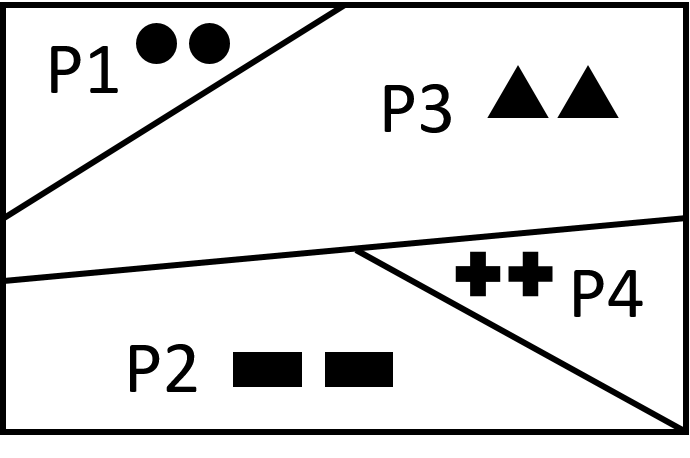
\includegraphics[width=1\linewidth]{Figures/networking2}
		\caption{Unknown correct game state when P3 joins the game.\\}
		\label{subfig:networking_ideal}
	\end{subfigure}
	\begin{subfigure}[t]{0.3\linewidth}
		\centering
		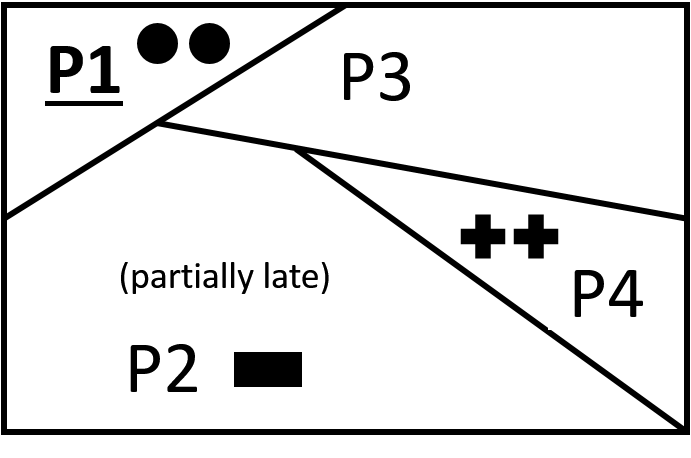
\includegraphics[width=1\linewidth]{Figures/networking1}
		\caption{Networking game state seen from the point of view of P1. P2 is partially synchronized, P4 is fully synchronized, and P3 is a new client that is late and is still sending its data}
		\label{subfig:networking_relative}
	\end{subfigure}
	
	
\end{figure}

\begin{figure}
	\centering
	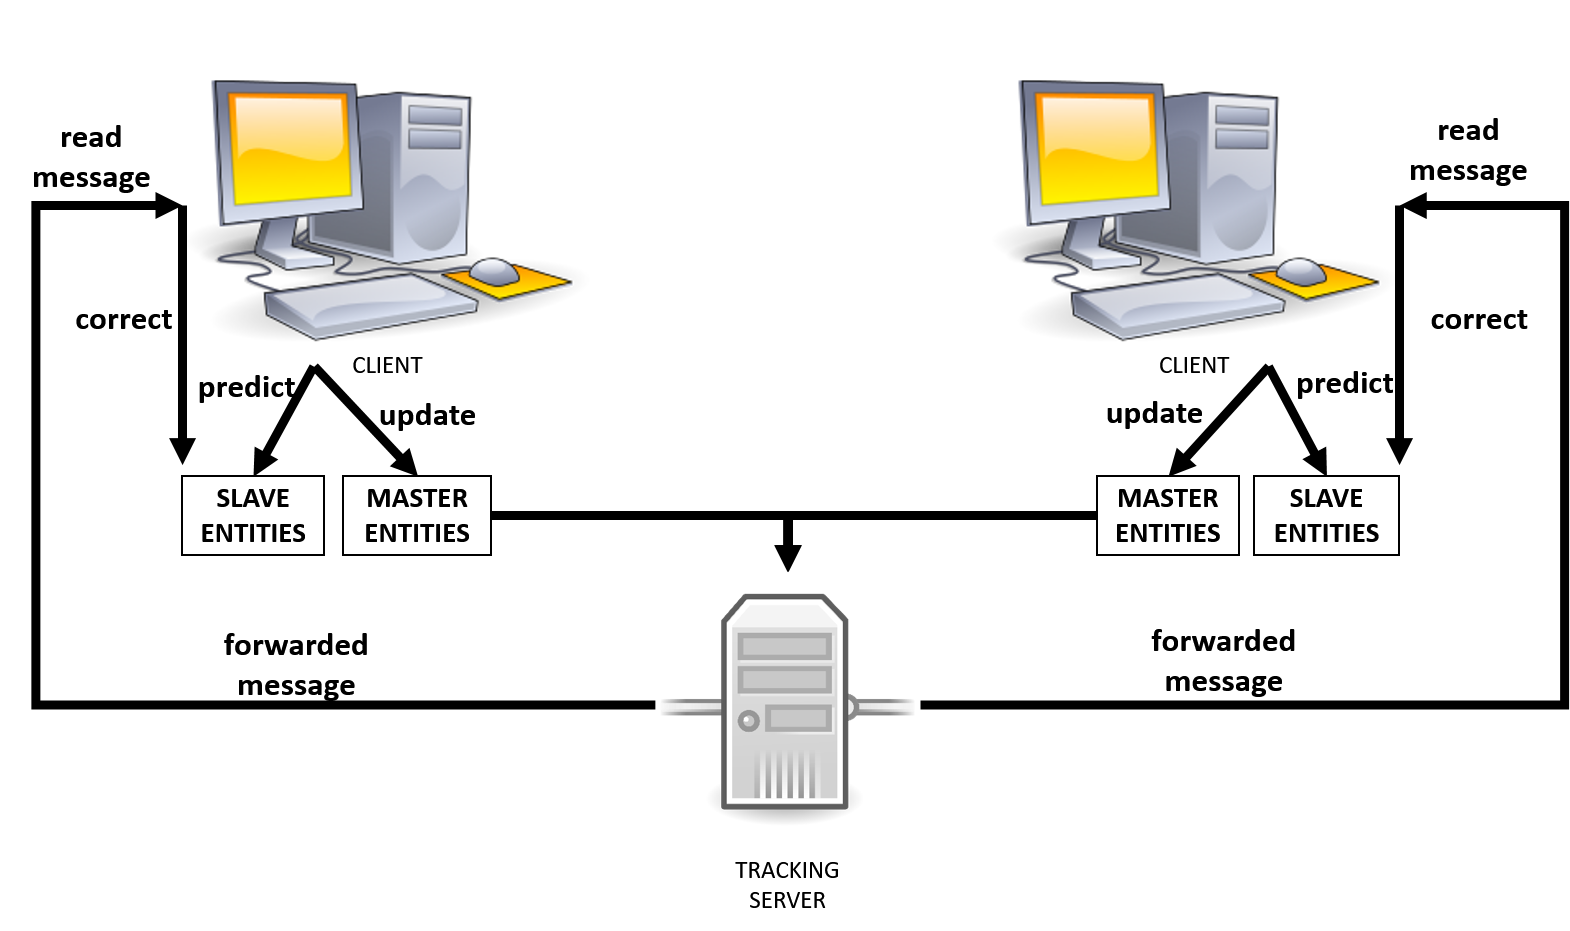
\includegraphics[width = \textwidth]{Figures/masterslave}
	\caption{master/slave architecture}
	\label{fig:masterslave}
\end{figure}

Note the aim of this architecture is to provide language-level primitives to describe the networking logic. This means that the compiler will be able to generate code compatible with the low-level network libraries that provide transmission functions over the network channel without having to change Casanova code in the program. In our implementation, we chose the .NET library \texttt{Lidgren}, which is widely used also in commercial game engines such as Unity3D and MonoGame, but nothing prevents the compiler to be expanded in order to target other similar libraries for other languages, such as jgroups \cite{ban2002jgroups}.

\section{Case study}
Let us consider a simple shooter game where each player controls a space ship. Players can move forward, backward, and rotate the ship to change direction. Moreover, they can use the ship lasers to shoot other players. If a laser hits an enemy ship, we increase the player's score. Designing such a game requires to address the following issues, depicted by the schematic representation in Figure \ref{fig:network_world}:

\begin{enumerate}
	\item Each player must maintain a local version of the game state (world). In order to avoid to flood the network with messages, all the copies are not fully synchronized at each frame, thus they are slightly different and each client knows the latest version of only part of the copy.
	\item A player \texttt{connecting} to an existing game must be able to receive the latest update of the game state and send the new ship he will control to existing players in the game.
	\item A player already \texttt{connected} to the game must detect a new connection and send his master portion of the game state.
	\item Each player must be able to control only one ship at a time. This means that the part of the game logic that processes the input and modifies the spatial data of the ship (position and rotation) should only be executed on the ship controlled by the player and not on the local copies of other players' ships. This means that each player sees as \texttt{master} only one ship instance.
	\item Each player must send the updated state of the ship he controls to the other players after executing the local update. To achieve better performance over the network, the data is not sent at every update, but with a lower frequency.
	\item Each player must receive the updated state of \texttt{slave} ships controlled by other players. In this phase, we must take into account that, as explained above, not every update is sent, so the player should ``predict'' what will happen during the game frames in which he does not receive an update.
\end{enumerate}

\section{Implementation}
\label{sec:ch_networking_casanova_networking_primitives}
Each of the scenarios described above requires specific language extensions. These extensions identify connection, ownership (master/slave), and various send and receive primitives. In this section, we introduce each primitive by using a multiplayer game example. We now give an implementation of the shooter game presented above, using the extended version of Casanova 2 with network primitives. The \texttt{world} contains a list of ships controlled by each player.
\begin{lstlisting}
world Shooter = {
Ships  : [Ship]
...
}
\end{lstlisting}

Each \texttt{Ship} contains a position, a rotation, a collection of shot projectiles, and the score.
\begin{lstlisting}
entity Ship = {
Position   : Vector2
Rotation   : float32
Projectiles : [Projectile]
Score		  : int
...
}

\end{lstlisting}

Each \texttt{Projectile} contains its position and velocity.

\begin{lstlisting}
entity Projectile = {
Position : Vector2
Velocity : Vector2
...
}
\end{lstlisting}

\subsubsection{Connection}
When a player connects, we must consider two different situations: (\textit{i}) a player is already in the game and must send the current game state to the connecting players, and (\textit{ii}) the player who is connecting needs to send the ship he will instantiate and control (its initial state). Both the players in the game and the connecting one must receive the game states that are sent. For this purpose we introduce two additional modifiers, \texttt{connecting} and \texttt{connected}, that can be added to rule declarations to mark their role in the multiplayer logic.

\paragraph{Connecting} A rule marked with \texttt{connecting} is executed once when a player joins the game for the first time. In our example, the player should send his initial state (the created ship) to the other players. We use the primitive \texttt{send\_reliable} because we must be sure that eventually all players will be notified of the ship creation.
\begin{lstlisting}
world Shooter = {
...
rule connecting Ships =
yield send_reliable Ships
}
\end{lstlisting}

\paragraph{Connected} A rule marked with \texttt{connected} is run whenever a new player joins the game by all existing players. When this occurs, each player sends its ship. The system will take care to send only the ship controlled locally by the player itself for each player. The rule will use the \texttt{send\_reliable} primitive for the same reason explained in the previous point.

\begin{lstlisting}
world Shooter = {
...
rule connected Ships =
yield send_reliable Ships
}
\end{lstlisting}

Note that even if the code is the same, the semantics of the two rules are different. The first one is executed by the player joining the game, who locally instantiates its \texttt{Ship} and must send its list of \texttt{Ships} (containing only the local instance) to the other players. The second one is executed by all existing players who must share with the joining player the list of existing ships.


\subsubsection{Master updates}
As explained above, each client manages a series of local game objects (called \textit{master objects}) that are under its direct control. The other clients read passively any update done on those instances and update their remote copy  (\textit{slave objects}) accordingly. We mark rules affecting the behaviour of master objects as \texttt{master}. In our example, the following situations are run as master: (\textit{i}) synchronizing the ships among players, (\textit{ii}) updating the ship and projectiles spatial data, and (\textit{iii}) creating and destroying projectiles.

\begin{enumerate}
	\item Each player is tasked to maintain the list of Ships in the world. This requires to receive the updated list from other players and to store the new value in a master rule. Indeed the world is a special case of an entity that is shared among players, and not directly owned by somebody. Each ship contained in that list and received from other players will be treated appropriately as slaves, while the only one owned by the current player will be under his direct control. In this rule we use \texttt{let!}, which is an operator that waits until the argument expression returns a result and then binds it to the variable. The symbol \texttt{@} stands for list concatenation. The rule uses \texttt{receive\_many}, which receives and collects the list of sent ships by the other players.
	
	\begin{lstlisting}
	world Shooter = {
	...
	rule master Ships =
	let! ships = receive_many()
	yield Ships @ ships
	}
	\end{lstlisting}
	
	\item The master version of the ship update reads the input of the player and moves (or rotates) the ship if the appropriate key is pressed. Note that this part must be executed only on a master object, because we want to allow each player to control only the ship he owns and instantiates at the beginning of the game. Below we show just the rule to move forward; the other movement and rotation rules are analogous. We use an \textit{unreliable send} because it is acceptable to lose an update of the position during a certain frame: shortly after, there will be a new update.
	
	\begin{lstlisting}
	entity Ship = {
	...
	rule master Position =
	wait world.Input.IsKeyDown(Keys.W)
	let vp = new Vector2(Math.Cos(Rotation), 
	Math.Sin(Rotation)) * 300.0f
	let p = Position + vp * dt
	yield send p
	}
	\end{lstlisting}
	
	We do the same for projectiles, except the projectile position is continuously updated and synchronized over the network without having to wait that a key is pressed.
	
	\item Creating a new projectile happens when the player shoots. A ship keeps track of the projectiles it has shot so far, and adds a new one to the list of the existing projectiles. The updated list is sent to all players with the new instance of the projectile (which is added as a new head of the list with the operator \texttt{::}). Here it is better to precise the semantics of the \texttt{yield} in conjunction with the use of networking primitives. A \texttt{yield} requires that the written value is type-compatible with the domain of the rule. Thus, when used with a \texttt{send} primitive, we must pass as argument a list. The system will ensure, for performance reasons, that the generated code only sends the new items added to the list. This semantics is defined as such for two main reasons: (\textit{i}) when sending the new projectiles we must also update the list in local (and given the immutability of Casanova we must replace the existing one), and (\textit{ii}) because in this way the programmer can focus on the logic of the game as if it were a single-player game without worrying of network-specific details. Note that the last \texttt{wait} forces the player to release the key before shooting again (semi-automatic fire). Removing that check would spawn multiple projectiles consecutively, which is not a wanted behaviour.
	
	\begin{lstlisting}
	entity Ship = {
	...
	rule master Projectiles =
	wait world.Input.IsKeyDown(Keys.Space)
	let vp = new Vector2(Math.Cos(Rotation), 
	Math.Sin(Rotation)) * 500.0f
	let projs = new Projectile(Position, vp) :: Projectiles
	yield send_reliable projs
	wait not world.Input.IsKeyDown(Keys.Space)
	}
	\end{lstlisting}
	
	Filtering the colliding projectiles and updating the score is run as a master rule. The rule computes the set difference between the ship projectiles and the colliding projectiles and updates the list of projectiles, sending them through the network as well. Even in this case, the network layer sends only the information about the projectiles to remove. Note that the score is managed by each player locally, as it does not require to be synchronized (we do not print the other players' scores. Doing so would indeed require to also send the score).
	
	\begin{lstlisting}
	entity Ship = {
	...
	rule master Projectiles, Score =
	let collidingProjs =
	[for p in Projectiles do
	let ships =
	[for s in Ships do
	where 
	s <> this and 
	Vector2.Distance(p.Position,s.Position) < 100.0f
	select s]
	where ships.Count > 0
	select p]
	let newProjectiles = Projectiles - collidingProjs
	yield send_reliable newProjectiles, 
	Score + collidingProjs.Count 
	}
	\end{lstlisting}
\end{enumerate}

\subsubsection{Managing remote instances}
The game objects that were not instantiated by a client, but received from another client, are \textit{slave objects} and must be synchronized differently than master objects. For this purpose, a rule can be marked as \texttt{slave}. In our example, we use slave rules in the following situations: (\textit{i}) synchronizing other players' ships and projectiles spatial data, and (\textit{ii}) projectiles instantiated by other players.

\begin{enumerate}
	\item Every remote projectile and ship is synchronized locally by a rule, which tries to \texttt{receive} a message containing updated spatial data. Below we provide the code to update the position of the ship; the synchronization of other spatial data is analogous.
	
	\begin{lstlisting}
	entity Ship = {
	...
	rule slave Position = yield receive()
	}
	\end{lstlisting}
	
	\item When a projectile is instantiated remotely, we have to receive it and add it to the list of projectiles. We use \texttt{receive\_many} because the new projectiles are added to a list. This case also supports the situation where a ship could shoot multiple projectiles at the same time.
	
	\begin{lstlisting}
	entity Ship = {
	...
	rule slave Projectiles =
	let! projs = receive_many()
	yield projs @ Projectiles
	}
	\end{lstlisting}
\end{enumerate}

In this scenario is important to discuss the atomicity of these transmissions: in the context of network games, reliability is often sacrificed for better network performance, so most of the data transmissions are unreliable (like in the case of the ship position). This means that we have no guarantee that the message will be received. Several issues can arise from this situation: for example, if a player fails to receive the position of the ship, then it might miss a collision with a projectile. This is a well-known issue in several shooter games and out-of-sync errors might happen during a multiplayer game. However, ensuring that all the data transmissions are reliable might affect network performance to the point that the game would become unplayable because of the network overload. 

Casanova 2 allows the programmer to decide whether the transmission should be reliable or not and experiment with the effect of a reliable transmission versus an unreliable one that does not overload the network. For example, the updated list of projectiles, after a collision, is always sent in a reliable way. This is acceptable because collisions are not so frequent. This is not true for the ship position, since movements are very frequent and mostly happen at every frame, thus it is something that should not be sent reliably at every frame.

Furthermore, we want to focus the attention on the implicit relationship between this networking architecture and the encapsulation: as shown for instance in the examples where the ship shoots a projectile, we ensure encapsulation by keeping a semantics that filters completely the details about networking. The programmer only worries about the logic of adding a new projectile, while the details of the network transmission are hidden. A hand-made implementation is usually prone to break this separation of concerns because the transmission logic is tightly coupled within the game logic itself.

\section{Entity update with functors in Metacasanova}
\label{sec:ch_networing_entity_update_functors}
In Section \ref{subsec:ch_mcnv_languages_casanova_semantics} we showed an implementation in Metacasanova of Casanova, a domain-specific language for game development, while in Section \ref{subsec:code_generation_discussion} we discussed about the reason of the poor performance of that implementation. In Chapter \ref{ch:functors} we extended Metacasanova with functors and modules to allow to embed the type system of an embedded  language \footnote{See the introduction of Chapter \ref{ch:functors} for a definition of this term} in the meta-compiler to overcome the problem of dynamic lookups at runtime. We then showed an implementation of records with modules and functors that significantly improved the performance of memory accesses, as shown in Section \ref{sec:ch_functors_evaluation}. In what follows we discuss another problem related to the implementation of Casanova and we provide an alternative implementation using functors that builds upon the existing implementation of records described in Section \ref{sec:ch_functors_record_implementation}.

\subsection{Casanova entity update}
\label{subsec:ch_networking_casanova_update}
In Section \ref{subsec:ch_mcnv_languages_casanova_semantics} we described the memory representation of a Casanova entity in Metacasanova and how the rules of an entity are updated. What was skipped for brevity was to describe how the system behind Casanova updates the entities of a Casanova program. As briefly described in Section \ref{sec:ch_mcnv_languages_casanova_language}, the structure of a program in Casanova is a tree, whose root is a special entity called \textit{World}. The world entity can contain fields that are instances of other entities as well, thus creating an additional level in the program tree. This is, of course, allowed also for regular entities, thus the height of the tree is arbitrary. Each entity might contain a set of rules that describe its dynamic behaviour with respect to time, thus they are updated by considering the time difference between the current and the previous update (\textit{frames}). Updating a rule is enforced by traversing the entity tree, thus when the field of an entity is an entity itself, the system will first update the entity instance contained in the field and then update the current entity. Casanova also natively supports lists and tuples as valid data types, and this requires to handle their update as well: a tuple or a list might themselves contain instances of entities that must be updated accordingly. In the case of a list of entities, we must run the update on each element, while in the case of a tuple we must examine each element and check whether it requires an update or not. This process is called \textit{update traversal} and might become very complex, as list and tuples can be combined together in infinite many ways, thus the process recursively calls the proper update depending on the type of the field.

At this purpose, let us consider a simulation consisting of an arbitrary amount of physical bodies, in the fashion of what was used in Section \ref{subsec:ch_functors_casanova_example}. The world entity will contain a list of physical bodies that are updated during the simulation. The Casanova code that described such a simulation is the following:

\begin{lstlisting}
worldEntity World {
	PhysicalBodies : [PhysicalBody]
}

entity PhysicalBody {
	Position				: Tuple<float,float>
	Velocity				: Tuple<float,float>
	Acceleration		: Tuple<float,float>
	
	rule Position = Position + Velocity * dt
	rule Velocity = Velocity + Acceleration * dt
}
\end{lstlisting}

\noindent
In this simulation, the update starts from \texttt{World}. This entity contains only one field, which is a list of physical bodies. Since \texttt{PhysicalBody} is an entity, the update must be run individually for each element of the list. The world contains no rules so after updating its only field we complete its update. At this point the update of each physical body examines each fields. All fields are represented as a point in a 2D space with a tuple containing two floating-point values. The update will examine each value of the tuple and find that they do not require any update (again because the only language abstractions that exhibit dynamic behaviours are entities). The update will then move on to run the rules that will update the content of \texttt{Position} and \texttt{Velocity}. The update process is sketched in Figure \ref{fig:ch_networking_simulation_update} and can thus be seen as a process that consists of the following steps:

\begin{enumerate}[noitemsep]
	\item An \textit{entity update} that traverses all the fields and rules of the entity and calls the appropriate updater.
	\item A \textit{field update} that is able to update (or not) the field depending on its type. The fields that will be updated have type \texttt{List}, \texttt{Tuple}, or \texttt{Entity}.
\end{enumerate}

\begin{figure}
	\centering
	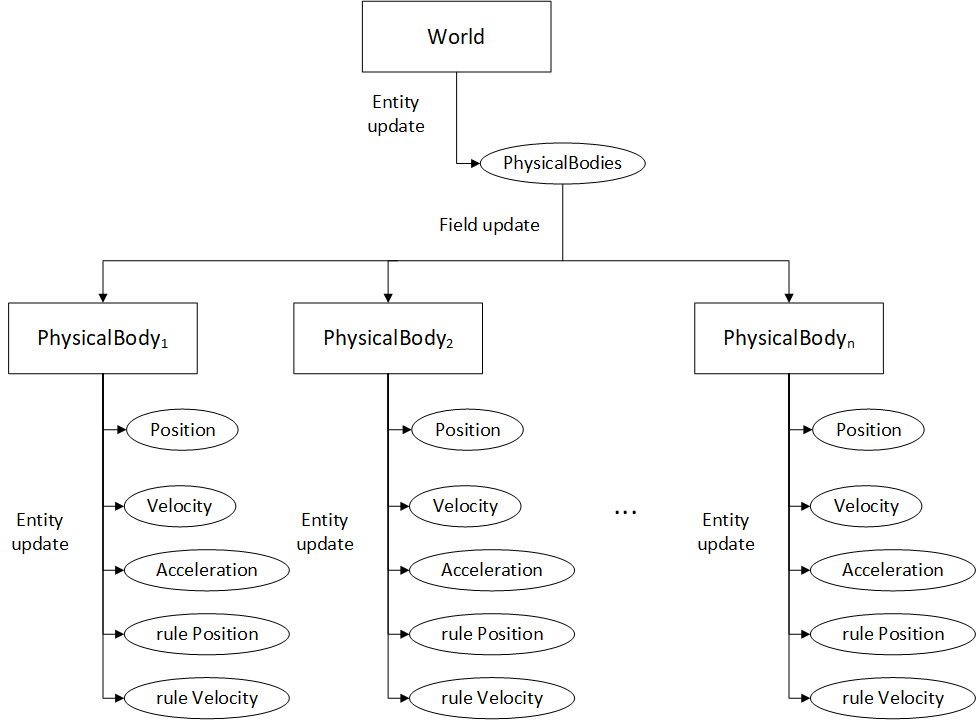
\includegraphics[width=\textwidth]{Figures/chapter_networking/update_traversal}
	\caption{Entity update for the simulation of physical bodies}
	\label{fig:ch_networking_simulation_update}
\end{figure}

\subsection{Update in Metacasanova}
\label{subsec:ch_networking_update_metacasanova}
The update mechanism described in Section \ref{subsec:ch_networking_casanova_update} can of course be integrated in the implementation of Casanova described in Chapter \ref{ch:languages}. In order to do so, we should dynamically look into the dictionary at each update, extract the field and perform an update according to the following cases:

\begin{itemize}[noitemsep]
	\item If the field is a list, then we must examine each element and choose for each one whether it needs to be updated or not. This is done by recursively applying these cases.
	\item If the field is a tuple, then we behave as above.
	\item If the field is an entity, then we must run an update on it.
	\item In all the other cases the field is not updated.
\end{itemize}

\noindent
The cases above are translated into four rules in Metacasanova. The first three will use pattern-matching to decide whether the examined field is a list, a tuple, or an entity. The fourth one is a default rule that simply returns the field as it is. Moreover, each entity should store a list of rules that are updated as well, where all the get and set operations require dynamic lookups in the symbol table of the entity.

Repeating the traversal of the entity tree at each update at runtime is unnecessary since

\begin{itemize}[noitemsep]
	\item The structure of a Casanova entity cannot change at runtime. Its fields and field types will always remain the same.
	\item The fields affected by an entity rule and the rules of an entity do not change during the program execution.
\end{itemize}

\noindent
This means that, by exploiting modules and functors, we are able to specify the structure of the update at compile time and generate directly the function that performs the update at runtime, in the same fashion of what had been done for the record setter and getter. In the following sections we will describe extensively the implementation of the update using modules and functors in Metacasanova that generates at compile time the functions necessary to perform the update of a Casanova program. Note that we will refer to the implementation of records given in Section \ref{sec:ch_functors_record_implementation}.

\subsection{Updater Modules}
\label{subsec:ch_networking_updater_modules}
As explained above, Casanova needs to recursively update fields that are lists, tuples, or entity instances. At this purpose, we define a module that represents an \textit{updatable element} in the Casanova language. The module constructor takes as only argument the type of the element to update. This module contains a function \texttt{update} that is able to update a value of this particular type and uses an additional parameter \texttt{dt} that contains the time difference between the current and the previous update. The function returns the updated value of the element. It also contains an utility functor for the 
 
\begin{lstlisting}
Module "ElementUpdater" => (elementType : *) : ElementUpdater {
	Functor "GetType" : *
	Func "update" -> elementType -> float : elementType
}
\end{lstlisting}

\noindent
The updater for a field is a module constructed by providing the record of the fields, its name as a string, and contains: (\textit{i}) an utility functor that returns the record used in the field updater, and (\textit{ii}) an update function that takes as input an instance of the record, \texttt{dt}, and returns the updated value of the field. We also define an external utility functor \texttt{GetFieldType} that can retrieve the type of a record field given the record it belongs to and its name. The rule for the functor calls the field getter and its \texttt{GetType} functor to retrieve the type of the name. This functor is used by the module constructor to correctly generate the return type of the \texttt{update} function.

\begin{lstlisting}
Functor "GetFieldType" => Record => string : *

GetField r name => getter
getter.GetType => type
---------------------------
GetFieldType r name => type

Module "FieldUpdater" => (r : Record) => (name : string) : FieldUpdater {
  Functor "GetRecord" : Record
  Func "update" -> r.RecordType -> float : (GetFieldType r name)
}
\end{lstlisting}

\noindent
Finally, the updater for a record is a module constructed by providing the record itself and contains: (\textit{i}) an utility functor that returns the type of the record, and (\textit{ii}) a function \texttt{update} that takes the instance of the record, \texttt{dt}, and returns an updated instance of the record.

\begin{lstlisting}
Module "RecordUpdater" => (r : Record) : RecordUpdater {
  Functor "RecordType" : *
  Func "update" -> r.RecordType -> float : r.RecordType
}
\end{lstlisting}

\subsection{Updatable elements}
\label{subsec:ch_networking_updatable_elements}
As explained above, the elements for which the update is needed can be lists, tuples, or entity instances. For this reason we have to create separately three different instances of the module \texttt{ElementUpdater} each one dedicated to updating one of those updatable elements. The first updatable element that we consider is an \textit{entity instance}. The module to update such updatable element uses a \texttt{RecordUpdater} to define how to entity instance should be updated. Indeed updating a field containing an entity instance requires to apply the specific updater for that entity, which in turn returns the updated instance of the entity itself. Thus the declaration for the functor that constructs the proper instance of the module for the entity updater is the following:

\begin{lstlisting}
Functor "UpdateEntity" => RecordUpdater : ElementUpdater
\end{lstlisting}

\noindent
The rule for this functor extract in its premise the type of the record by calling the utility functor \texttt{RecordType} in the record updater passed as parameter to the constructor of the module. The \texttt{update} function uses the record updater to recursively update the entity instance in its premise and then returns the result of this update.

\begin{lstlisting}
recordUpdater.RecordType => recordType
--------------------------
UpdateEntity recordUpdater => ElementUpdater recordType {

	----------------------
	GetType => recordType
 
  recordUpdater.update entity dt -> entity'
  ------------------------------
  update entity dt -> entity'
}
\end{lstlisting}

\noindent
The second updatable element is the list. An updater for a list must take the updater for its elements. Since a list contains elements of the same type, only one updater is required to instantiate its updater module. The functor \texttt{UpdateList} used to generate this module takes one argument which is an \texttt{ElementUpdater}. This is done because the elements of a list could be themselves other lists, entities, or tuples, so we must be able to use their updaters as arguments for this function. The declaration for this functor is thus:

\begin{lstlisting}
Functor "UpdateList" => ElementUpdater : ElementUpdater
\end{lstlisting}

\noindent
The rule for \texttt{UpdateList} extracts in its premise the type of the elements of the list by calling the functor \texttt{GetType} in the element updater provided as input. It then instantiates an \texttt{ElementUpdater} with the type \texttt{List} using as argument for the generic type the type of the element extracted in its premise. The \texttt{update} function for the list is recursive: its base case is the empty list, for which it simply returns an empty list. For a non-empty list the rule for this function uses the element updater in its premise to update the head of the list and then recursively calls the \texttt{update} of the list on the tail to updater the remaining part.

\begin{lstlisting}
updater.GetType => elementType
---------------------------------
UpdateList updater => ElementUpdater List[elementType] {

  -----------------
  GetType => List[elementType]

  --------------------
  update nil dt -> nil

  updater.update x dt -> x'
  update xs dt -> xs'
  -------------------
  update (x :: xs) dt -> (x' :: xs')
}
\end{lstlisting}

\noindent
The updater for tuples is built by defining a functor that takes as input two element updaters, one for the current element of the tuple, and one for the second one. Note that it is possible to recursively provide a tuple updater as a second updater to support the update of tuples containing more than two elements. For example, the updater for \texttt{Tuple[PhysicalBody,Tuple[PhysicalBody,\\PhysicalBody]]} would require to pass an entity updater and recursively a tuple updater. The declaration of this fuctor is thus:

\begin{lstlisting}
Functor "UpdateTuple" => ElementUpdater => ElementUpdater : ElementUpdater
\end{lstlisting}

\noindent
The rule for \texttt{UpdateTuple} uses in its premises \texttt{GetType} from the first updater and the second updater to obtain the types of the first and second element of the tuple. It then instantiates \texttt{ElementUpdater} with the tuple type called with the type of the first and second element as arguments for the generics. The \texttt{update} function runs the \texttt{update} of the first updater on the first element of the tuple and the second updater on the second element.

\begin{lstlisting}
updater.GetType => firstType
nextUpdater.GetType => nextType
---------------------------------------------
UpdateTuple updater nextUpdater => ElementUpdater Tuple[firstType,nextType] {

  -------------------
  GetType => Tuple[firstType,nextType]

  updater.update x dt -> x'
  nextUpdater.update x' dt -> xs'
  ----------------------
  update (x,xs) dt -> (x',xs')
}
\end{lstlisting}

Finally, we need a \texttt{ZeroUpdate} that is required for fields whose values do not change with respect to time, namely all those that do not fall in the three categories above. The functor \texttt{ZeroUpdate} takes as input any type and builds an \texttt{ElementUpdater} with that type. The rule for \texttt{update} simply returns the value of the field as it is.

\begin{lstlisting}
Functor "ZeroUpdate" => * : ElementUpdater

-----------------------
ZeroUpdate type => ElementUpdater type {

  ----------------
  GetType => type

  ----------------
  update v dt -> v
}
\end{lstlisting}

\subsection{Updatable Fields and Records}
The field updater is instantiated by a functor that takes as input an element updater, a record containing the field, and the name of the field to update. Its declaration is the following:

\begin{lstlisting}
Functor "UpdateField" => ElementUpdater => Record => string : FieldUpdater
\end{lstlisting} 

\noindent
The rule for the \texttt{update} function creates in its premises a field getter through the record and the field name passed as input. It then call the function \texttt{get} of the getter with the record instance taken as input to get the value of the field. It then uses the \texttt{update} function from the element updater taken as input from the functor to update the field.

\begin{lstlisting}
----------------------------------------
UpdateField elementUpdater r name => FieldUpdater r name {

  ---------------
  GetRecord => r

  GetField r name => getter
  getter.get rec -> field
  elementUpdater.update field dt -> field' 
  -----------------------------
  update rec dt -> field'
}
\end{lstlisting}

\noindent
The record updater is built by a functor \texttt{Update} that takes as input a field updater, a record updater to update the next part of the record, and returns an instance of the \texttt{RecordUpdater} module. The rule that evaluates the functor extracts the record from the field updater in its premise and passes it to the module constructor for the record updater. The rule for \texttt{update} generates a setter for the field by using the record and the field name. It then calls the field updater passing the record instance and \texttt{dt} as input. This premise will return the updated value for the field. The following premise uses the \texttt{set} function from the previously generated setter to update the record with the new value of the field. After this step it calls the \texttt{update} function of the record updater passed as function argument, which is recursively able to update the remaining part of the record. The result of this update is then returned as final result. Both the functor declaration and the rule for it are provided below

\begin{lstlisting}
Functor "Update" => FieldUpdater => RecordUpdater : RecordUpdater

fieldUpdater.GetRecord => r
---------------------------
Update fieldUpdater nextUpdater => RecordUpdater r {

  r.RecordType => recordType
  ------------------------
  RecordType => recordType

  SetField r name => setter
  fieldUpdater.update rec dt -> v
  setter.set rec v -> rec'
  nextUpdater.update rec' dt -> updatedRecord
  ----------------------------
  update rec dt -> updatedRecord
}
\end{lstlisting}

\noindent
Note that it is possible to provide different field updaters for the same field, as it is possible that, besides the standard Casanova traversal, one wants to define a custom way of updating the field through a Casanova rule.

In order to stop this otherwise infinite recursive process, we must also generate a record updater that simply returns the record as it is. We build such updater through the functor \texttt{NoUpdate}. This functor takes as input a record and instantiates its updater with it. The updater contains a rule for the \texttt{update} function that simply returns the record as it is. The implementation for this updater is provided below:

\begin{lstlisting}
Functor "NoUpdate" => Record : RecordUpdater

---------------------
NoUpdate r => RecordUpdater r {

  r.RecordType => recordType
  ----------------------
  RecordType => recordType
  
  ----------------
  update r dt -> r
}
\end{lstlisting}

\noindent
Finally, rules can be implemented as a field updater that is instantiated by a functor taking as input the record and the field name. The \texttt{update} function will contain the specific code that the rule will perform. In the following section we will provide the implementation of the physical body simulation and show how to use functors to generate the field updater for rules.

\subsection{Physical Body Simulation with Functors}
\label{subsec:ch_networking_simulation}
In this section we present the implementation with functors of the simulation in Casanova presented in Section \ref{subsec:ch_networking_casanova_update}. The simulation consists of a set of bodies that moves according to their physical properties. As previously done in Section \ref{sec:ch_functors_record_implementation}, we create a functor that builds the record module instance for the physical body:

\begin{lstlisting}
Functor "PhysicalBodyType" : Record

RecordField "Acceleration" Tuple[float,float] EmptyRecord => acceleration
RecordField "Velocity" Tuple[float,float] acceleration => velocity
RecordField "Position" Tuple[float,float] velocity => body
---------------------------
PhysicalBodyType => body
\end{lstlisting}

\noindent
At this point, we define the updaters for the physical body fields. Its fields consist of a tuple with two floating point values. Since floating-point values do not require to be updated in Casanova, we create an updater for the floating-point numbers by using the \texttt{ZeroUpdate} functor that instantiates \texttt{ElementUpdater} with an \texttt{update} function that simply returns the input value.

\begin{lstlisting}
Functor "FloatUpdater" : ElementUpdater

ZeroUpdate float => zero
--------------------------
FloatUpdater => zero
\end{lstlisting}

\noindent
\texttt{ZeroUpdate} calls \texttt{ElementUpdater} with \texttt{elementType := float}. The instance of this module will then contain the following functor rule and function declaration\footnote{Note that the evaluation rules in a functor are always the same for each instance of a module, so from now on we omit them for brevity}.

\begin{lstlisting}
Func "update" -> float -> float : float

-----------------
GetType => float
\end{lstlisting}

\noindent
At this point we can define the element updater for the \texttt{Tuple} that contains the floating point values. This time we use the functor \texttt{UpdateTuple} to instantiate the \texttt{ElementUpdater} module by passing twice \texttt{FloatUpdater} to it. When we do so, we have that (see the definition of the rule for this functor):

\begin{lstlisting}
updater := FloatUpdater
nextUpdater := FloatUpdater
firstType := updater.GetType := float
nextType := nextUpdater.GetType = float
\end{lstlisting}

\noindent
Thus \texttt{ElementUpdater} will be called with \texttt{elementType := Tuple[float,float]}. This module instance will then contain the following functor rule and function declaration:

\begin{lstlisting}
Func "update" -> Tuple[float,float] -> float : Tuple[float,float]

-----------------------------
GetType => Tuple[float,float]
\end{lstlisting}

\noindent
We now build the field updaters for the two Casanova rules of the physical body. In order to do so, we define two functors that build their field updaters:

\begin{lstlisting}
Functor "PositionRule" : FieldUpdater
Functor "VelocityRule" : FieldUpdater
\end{lstlisting}

\noindent
\texttt{PositionRule} will instantiate \texttt{FieldUpdater} in the following evaluation rule:

\begin{lstlisting}
--------------------------------
PositionRule => FieldUpdater PhysicalBodyType "Position" {

  ---------------------
  GetRecord => PhysicalBodyType

  getPos body -> (xp,yp)
  getVel body -> (xv,yv)
  <<xp + xv * dt>> -> xp'
  <<yp + yv * dt>> -> yv'
  ---------------------------
  update body dt -> (xp',yp')
}
\end{lstlisting}

\noindent
Note that \texttt{getPos} and \texttt{getVel} are functions able to retrieve respectively the position and velocity from a physical body, analogously to what was done in Section \ref{sec:ch_functors_record_getter}. The \texttt{update} function uses these two functions in its premises to retrieve the value of the position and velocity and then updates the position according to the differential equation described in Section \ref{subsec:ch_functors_casanova_example}. The update for the velocity field is done analogously:

\begin{lstlisting}
--------------------------------
VelocityRule => FieldUpdater PhysicalBodyType "Velocity" {

  --------------------
  GetRecord => PhysicalBodyType

  getVel body -> (xv,yv)
  getAcc body -> (xa,ya)
  << xv + xa * dt >> -> xv'
  << yv + ya * dt >> -> yv'
  ---------------------------
  update body dt -> (xv',yv')
}
\end{lstlisting}

\noindent
We now have all the necessary tools to create the whole updater for a physical body. This updater is built by calling \texttt{UpdateTuple} to generate the updater for the tuple element representing the vector. This updater is used in all three field updaters for the physical body. We also use \texttt{PositonRule} and \texttt{VelocityRule} to create the correct updater for the two rules of the physical body.

\begin{lstlisting}
UpdateTuple FloatUpdater FloatUpdater => vectorUpdater
UpdateField vectorUpdater PhysicalBodyType "Position" => posUpdate  
UpdateField vectorUpdater PhysicalBodyType "Velocity" => velUpdate  
UpdateField vectorUpdater PhysicalBodyType "Acceleration" => accUpdate
NoUpdate PhysicalBodyType => zero
Update VelocityRule zero => velRule
Update PositionRule velRule => posRule
Update accUpdate posRule => accFieldUpdate
Update velUpdate accFieldUpdate => velFieldUpdate
Update posUpdate velFieldUpdate => bodyUpdater
--------------------------
BodyUpdater => bodyUpdater
\end{lstlisting}

\noindent
The first premise of this functor rule creates the updater for the vecotr. From premise 2 to premise 4 we create the updater for the three fields of the physical body. Premise 5 calls \texttt{NoUpdate} to build the module that terminates the update of the record. From Premise 6 on we build the record updaters necessary to update all the fields and rules of the physical body and then we assemble them together.
Let us now consider the following physical body instance

\begin{lstlisting}
(1.0,1.0),((0,0,0.0),((3.0,3.0),()))
\end{lstlisting}

\noindent
and let us see what happens when we call the \texttt{update} function of the \texttt{BodyUpdater}. The function will invoke the tuple updater which returns the tuple as it is, set the field to this value (which does not change), and recursively call \texttt{update} from the next updater. The following two updaters are the same, so the effect is identical. The updater for the position rule will instead run the \texttt{update} code of the module instance generated by the rule functor and update the field of the record accordingly. This will generate a record instance containing the field with the updated value. This new record instance is then recursively passed to the next \texttt{update} call where the \texttt{update} of the module instance generated by the rule functor for velocity is invoked. The updated record is then returned in an analogous way. At this point the \texttt{update} of the module instance generated by \texttt{NoUpdate} is called, which simply returns the record as it is.

We now repeat the same process to define the world entity. We thus define a functor to build the record for the world, which contains a single field that is a list of physical bodies.

\begin{lstlisting}
Functor "WorldType" : Record

RecordField "PhysicalBodies" List[PhysicalBodyType] EmptyRecord => world
---------------------------------
WorldType => world
\end{lstlisting}

\noindent
The updater for the world simply uses the \texttt{BodyUpdater} functor generated above to build a record instance that contains the update function for a physical body. It then builds a list updater passing as argument \texttt{BodyUpdater} (note that this is correct as this functor accepts a record updater as parameter).

\begin{lstlisting}
Functor "WorldUpdater" : RecordUpdater

UpdateEntity BodyUpdater => bodyUpdater
UpdateList bodyUpdater => listUpdater
UpdateField listUpdater WorldType "PhysicalBodies" => fieldUpdater
NoUpdate WorldType => zero
Update fieldUpdater zero => worldUpdater
--------------------------------------
WorldUpdater => worldUpdater
\end{lstlisting}

\noindent
The rule for the functor creates in its first premise an entity updater by passing the updater for the physical body. This updater allows to update each element in the list of physical bodies stored in the world entity. The second premise creates an updater for the whole list by passing the entity updater created at the previous step. This updater instantiates a module that is able to traverse the whole list and update each element by means of the entity updater. The third premise creates a field updater for \texttt{PhysicalBodies} by using the list updater, and the fourth creates as usual a \texttt{NoUpdate} to stop the update process. Finally, the last premise assembles the two field updaters into a record updater for the world entity. At this point, in order to update the world entity, it is enough to call this functor and access the \texttt{update} function for the world record.

We think it is worthy of note that all the updaters presented so far are built at compile time and that the only component that will be generated in the target code is the \texttt{update} function. This means that we get rid of all the dynamic lookups, described in Section \ref{subsec:ch_networking_update_metacasanova} in the entity field introduced in Section  to inspect the type of the field itself and decide whether or not we require to perform the recursive update process on it. The update traversal with functors is instead generated at compile time, thus the structure of the update is pre-computed during the compilation step, and its execution delegated at runtime. This is possible because the structure of the update does not change with the execution of the program.

\subsection{Interruptible rules with functors}
\label{subsec:ch_networking_interruptible_rules}
With what shown so far, we can implement the update traversal of the fields of a Casanova entity and we can implement Casanova rules as updaters that act on the fields of an entity. However, we have not described yet how to implement the mechanism of rule interruption described in Section \ref{subsec:ch_mcnv_languages_rule_evaluation}. At this purpose, we have to refactor the implementation of the updaters seen so far: we assume that now the record field of a Casanova entity contains not only the value but a list of statements that represent the continuation of its rule, which represents the code left to execute after the rule is paused. The continuation will have type \texttt{stmt}, where \texttt{stmt} is a meta-data structure representing a statement in Casanova like shown in Section \ref{subsec:ch_mcnv_languages_rule_evaluation}. The reader should keep into account that we can compose a sequence of statements through the \texttt{;} operator introduced in the same section. The field updater must be refactored as well: its update function now does not only return the updated field value but also the continuation of the rule:

\begin{lstlisting}
Module "FieldUpdater" => (r : Record) => (name : string) : FieldUpdater {
  Functor "GetRecord" : Record
  Func "update" -> r.RecordType -> float : Tuple[(GetFieldType r name),stmt]
}
\end{lstlisting}

\noindent
In this way we are correctly able to generate the declaration of the update function depending on the type of the field and, at the same time, to store the updated continuation of the rule. We now define a new functor called \texttt{Coroutine} that generates an instance of a field updater. The instantiation of the module should also contain a function \texttt{tick} that is able to correctly process the continuation of the rule and, when its body has been fully evaluated, to restart from the beginning. It should also contain a definition of the evaluation rules of all the Casanova statements introduced in Section \ref{subsec:ch_mcnv_languages_rule_evaluation}. For brevity here we show only how to re-implement \texttt{wait}, \texttt{when}, and \texttt{yield}, all the others can be adjusted analogously to those. The following is the declaration of the Coroutine functor:

\begin{lstlisting}
Functor "Coroutine" => Record => string => stmt : FieldUpdater

----------------------------
Coroutine r name stmts => FieldUpdater r name {
  ... 
  // see the implementation below
}
\end{lstlisting}

\noindent
This functor takes the record and the name of the fields the rule is updating, as well as a list of statements that represents the body of the coroutine and produces a field updater enriched with the utility functions mentioned above (remember that a module instance must contain the implementation of at least all the declarations provided in the module declaration). From now on we provide the snippets of the implementations in the module in isolation, but the reader should keep in mind that they are defined within the scope of the module instance. The first function that we implement is \texttt{update}. This function is almost identical from the version described in Section \ref{subsec:ch_networking_simulation}, but this time the getter of the field will return both the value and the continuation of the rule built so far. We then call a \texttt{tick} function (see below) that is able to process the continuation of the rule. This function in general produces a pair containing the updated field value (when we encounter a \texttt{yield} statement) and the new continuation produced by the current execution of the rule. Note that the implementation of \texttt{update} is correctly able to return a pair because it has been redefined above in the new version of \texttt{FieldUpdater}.

\begin{lstlisting}
GetField r name => getter
getter.get body -> (v,k)
tick entity k dt -> (v',k')
-------------------------
update entity dt -> (v',k')
\end{lstlisting}

\noindent
The \texttt{tick} function takes a record instance as input, a list of statements, and \texttt{dt} and returns the pair of value and continuation produced by the evaluation of the rule body. The function calls \texttt{eval\tu s} that is similar to the homonym function presented in Section \ref{subsec:ch_mcnv_languages_rule_evaluation}, with the difference that it now returns a pair of value field and list of statements compatible with the required result.

\begin{lstlisting}
Func "tick" -> r.RecordType -> List[stmt] -> float : Tuple[r.RecordType,List[stmt]]
Func "eval_s" -> r.RecordType -> stmt -> float : Tuple[r.RecordType,stmt]


eval_s entity stmts dt -> res
--------------------------
tick entity nop dt -> res

eval_s entity statements dt -> (v,(atomic;k))
tick entity k dt -> res
-----------------------------------
tick entity statements dt -> res

eval_s entity statements dt -> res
-----------------------
tick entity statements dt -> res
\end{lstlisting}

\noindent
The function \texttt{tick} comes in three versions: the first one is executed when the rule has completed its execution and the body of the original rule should be rebuilt. In this case the function simply calls \texttt{eval\tu s} with the statements provided as argument of the functor \texttt{Coroutine}. The second one is when we evaluate an atomic statement: at this purpose we introduce a placeholder statement \texttt{atomic} that is returned in the continuation after an atomic statement has been evaluated. This case forces \texttt{tick} to be immediately re-evaluated without interrupting the rule execution. The third case happens when the rule evaluation has previously produced a continuation. In this case we pass the continuation instead of the original body of the rule to \texttt{eval\tu s}.

The function \texttt{eval\tu s} is very similar to its old counterpart, but this time it returns the pair of value and continuation resulting from the evaluation of the first statement in the current rule continuation. In the case of an empty continuation (the only statement is \texttt{nop}) then we return an empty continuation. The field of the value is unchanged so we use its getter to retrieve the value an return it in the result.

\begin{lstlisting}
GetField r name => getter
getter.get entity -> (v,cont)
-------------------------------
eval_s entity nop dt -> (v,nop)
\end{lstlisting}

We now proceed to describe how \texttt{wait} and \texttt{yield} behaves. \texttt{wait} as usual simply checks whether the timer has elapsed. If that is the case, then it returns the continuation preceded by an \texttt{atomic} statement to force the immediate re-evaluation in \texttt{tick}. Otherwise it updates the timer by subtracting \texttt{dt} seconds and builds another \texttt{wait} statements that is placed in the continuation. In both cases the statement returns the current value of the field the rule is updating because it is untouched in the semantics of \texttt{wait}.

\begin{lstlisting}
t <= 0.0
GetField r name => getter
getter.get entity -> (v,cont)
---------------------------------------------
eval_s entity (wait t;k) dt => (v,(atomic;k))

t > 0.0
GetField r name => getter
getter.get entity -> (v,cont)
<<t - dt>> -> t'
---------------------------------------------
eval_s entity (wait t;k) dt => (v,(wait t';k))
\end{lstlisting}

\noindent
Note that the correct \texttt{getter} is generated at compile time, so the overhead of accessing the field value is minimal as shown in Section \ref{sec:ch_functors_evaluation}. The statement \texttt{when} behaves in the very same way, except that this time 


Finally \texttt{yield} simply evaluates the expression whose value is used to set the field and then returns it in the result of the evaluation. Note that we use the function \texttt{eval} already described in the first implementation of Casanova in Metacasanova. The behaviour of this function is exactly the same, except that now, if we need to retrieve the value of a specific field for the computation of the expression result, we can use the \texttt{GetField} functor to build the appropriate getter and thus save on performance. Also note that the statement evaluation does not set the field itself, but as seen before it delegates this operation to the record updater. This is because the result of calling the setter on a record returns the updated record instance and not a value compatible with the field. Note also that the evaluation of \texttt{yield} does not produce \texttt{atomic} like for \texttt{wait} because according to Casanova semantics the \texttt{yield} stops the rule execution for one frame.

\begin{lstlisting}
eval entity expr -> v
--------------------------------
eval_s (yield expr;k) dt -> (v,k)
\end{lstlisting}

\noindent
It is worthy of note that, having placed the semantics of Casanova in a module instantiation, the language is able to build ad-hoc semantics for each specific field that we need to update through the rule. In other words, calling the coroutine functor with a specific field produces a different version of the language semantics at compile time, where the statements that need to access the value of the field contain directly the getter of that field generated at run-time. This allows us to incorporate the benefits of the record lookup optimization described in Chapter \ref{ch:functors} in the language semantics.

The final modification that we need to implement is on the record updater. The record updater now receives the pair of field value and rule continuation that must be stored in the field after its update. The updater uses the new generated pair to update both the field value and its rule continuation. This continuation will be used at the next update to evaluate the remaining part of the rule

\begin{lstlisting}
fieldUpdater.GetRecord => r
---------------------------
Update fieldUpdater nextUpdater => RecordUpdater r {

  r.RecordType => recordType
  ------------------------
  RecordType => recordType

  SetField r name => setter
  fieldUpdater.update rec dt -> (v,k)
  setter.set rec (v,k) -> rec'
  nextUpdater.update rec' dt -> updatedRecord
  ----------------------------
  update rec dt -> updatedRecord
}
\end{lstlisting}

\subsubsection{Multiple rules updating the Same Field and Local variables}
To conclude this section we want to point out that, in the implementation of interruptible rules described above, we implicitly make the assumption that only one rule is updating each field of the record. Indeed the rule continuation is saved in the field itself, thus if multiple rules are affecting the same field we would need to store their continuations separately, which is not possible in the current implementation. A naive approach would be to allow to store a list of statements, one for each rule acting on that field, where each element is the continuation of a specific rule. This approach affects the performance because we would need to iterate the whole list every time we need to update a rule. Since the number of rules updating a field does not change at run time, we can instead use a record to store their continuations whose structure is provided at compile time. In this way it will be possible to retrieve the continuation of a rule just by using a getter that is generated at compile time. Here we just briefly sketch the implementation for brevity. A schematic representation of the implementation can also be seen in Figure \ref{fig:ch_networking_interruptible_rules}.

\begin{figure}
  \centering
  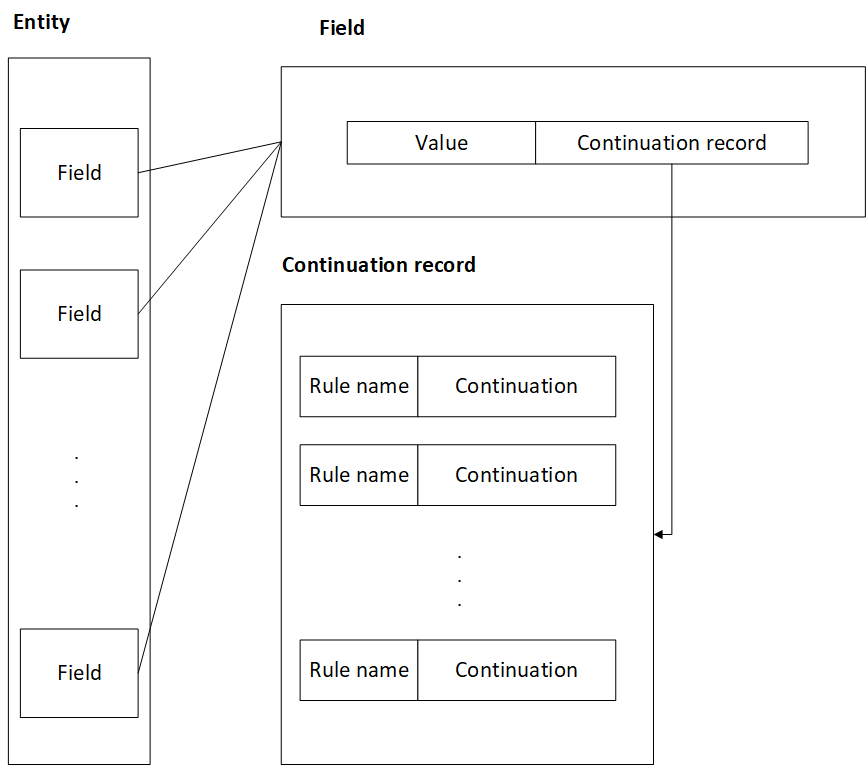
\includegraphics[width=\textwidth]{Figures/chapter_networking/interruptible_rules}
  \caption{Schematic representation of the implementation of the interruptible rules}
  \label{fig:ch_networking_interruptible_rules}
\end{figure}

A field of the entity record must be adapted now to contain not only the field value, but a record instance used to store the continuations of the Casanova rules affecting that field. Since a record requires a name for each field, we can expand the coroutine functor to take a string representing an identifier for each rule and the continuation record itself:

\begin{lstlisting}
Functor "Coroutine" => string => Record => Record => string => stmt : FieldUpdater


---------------------------
Coroutine ruleId continuation r name => FieldUpdater r name {
  ...
}
\end{lstlisting}

\noindent
Now the first string in the declaration of the functor represents the rule identifier, while the other arguments have the same semantics (record and field of the record the rule can modify). When a Casanova statement requires to store the continuation it can use \texttt{ruleId} to build the setter for the record field of the continuation record. It then calls the function \texttt{set} from the setter module instance to save the continuation of each rule. In this way every rule acting on the record is able to store separately its continuation in the continuation record. As an example, we provide below the evaluation rule for the \texttt{wait} statement that updates the continuation in this implementation:

\begin{lstlisting}
eval entity expr -> t
t > 0.0
GetField r name => getter
getter.get entity -> (v,cont)
SetField cont ruleId => continuationSetter
continuationSetter.set (wait(t - dt);k) -> cont'
---------------------------------------------
eval_s entity (wait t;k) dt => (v,cont')
\end{lstlisting}

\noindent
Another aspect that has not been considered yet is how to define variables local to the rule (local bindings). Since the set of local bindings is known at compile time, we can modify the continuation record to store not only the continuation itself, but also the state of the local bindings as record of bindings. In this way an element of the continuation record, that we can now call rule state, stores not only the statements of the rule left to evaluate but also the state of the local bindings. When we need to read the value of a binding or update it, we can again use a getter or setter by accessing the rule state and getting or setting the appropriate field for the binding from the binding record. A schematic representation of this implementation can be seen in Figure \ref{fig:ch_networking_interruptible_rules_with_state}.

\begin{figure}
  \centering
  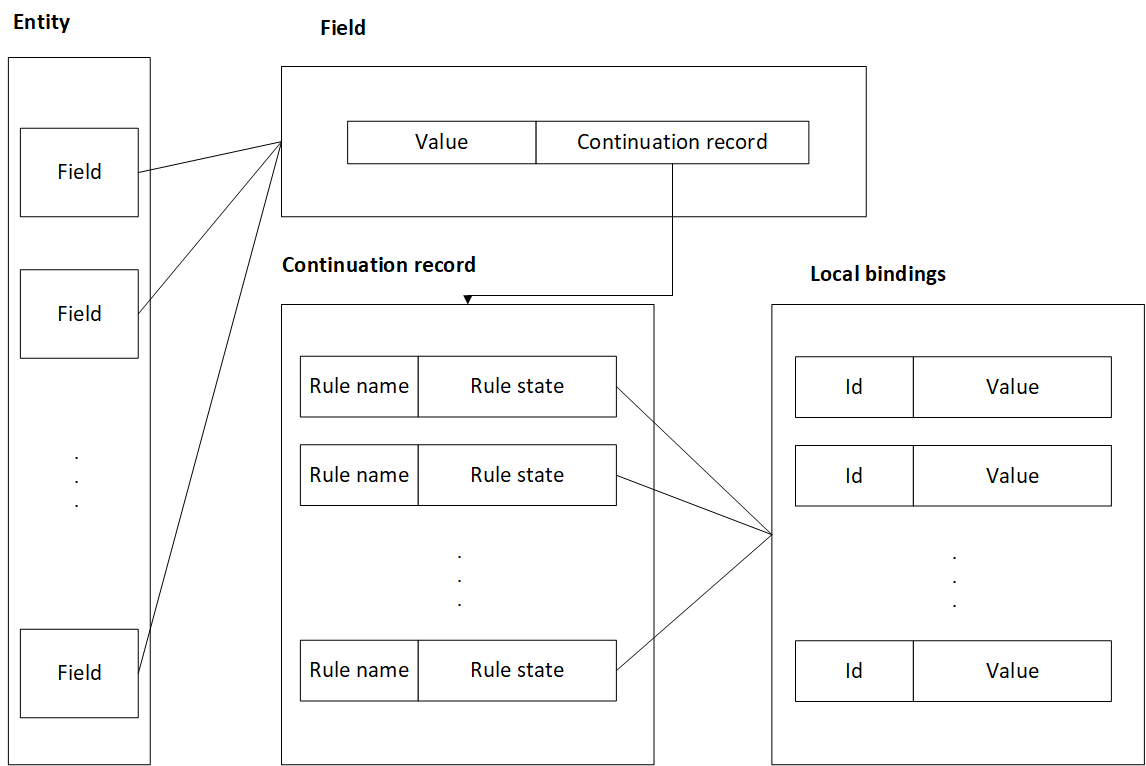
\includegraphics[width=\textwidth]{Figures/chapter_networking/interruptible_rules_with_state}
  \caption{Schematic representation of the implementation of interruptible rules with local bindings}
  \label{fig:ch_networking_interruptible_rules_with_state}
\end{figure}

As final remark, we point out that the use of records to store the rule continuations and local bindings show how the record optimization introduced in Chapter \ref{ch:functors} can also be adapted to implement a generic symbol table to store various information regarding the language elements that are needed during the execution of the generated code, thus making this approach extremely flexible for different situations.

\subsection{Evaluation}
\label{subsec:ch_networking_evaluation}
In the previous sections we showed how to use functors to implement the entity update traversal of the domain-specific language for game development Casanova. Based on the preliminary analysis performed in Chapter \ref{ch:functors}, we claimed that using functors would improve the performance of the implementation of Casanova in Metacasanova given in Chapter \ref{ch:languages} by, at the same time, inlining the access to the entity fields and pre-building the traversal for the Casanova program at compile time, instead of dynamically accessing the fields from a dictionary and inspecting their type to perform the update traversal at every update. In this section we show the experimental results that show the performance of this implementation in comparison to the first dynamic implementation presented in Chapter \ref{ch:languages}.

\subsubsection{Experimental Setup}
For this evaluation we have implemented the physical body simulation that was presented in the previous sections. The simulation has been run for 10000 frames, which roughly correspond to 3 minutes assuming an average update rate of 60 frames/second, with a number of physical bodies ranging from 100 to 1000. Each physical body is randomly generated, that is, its initial position, velocity, and acceleration is randomly generated. We measured the time at the beginning and at the end of the execution of the whole simulation and we averaged the total time by the number of frames the simulation has been running for. We then compared the result with what obtained for the implementation shown in Chapter \ref{ch:languages}.

\subsubsection{Results}
In Table \ref{tab:ch_networking_evaluation} we can see that the update time is in the order of milliseconds or one tenth of milliseconds where the dynamic implementation was in the order of one hundredth of seconds with 1000 entities. This corresponds roughly to a frame rate of 939 frames/second for the functor implementation versus 28 frames/second. The performance gain ranges from a maximum of 55.397 to a minimum of 33.117 times with an avarage gain of 42.508 times. This comes with no surprise, since in Section \ref{sec:ch_functors_evaluation} we tested the gain of accessing record fields with the functor implementation compared to the dynamic tables, and we had an average gain of roughly 11 times. The gap with the dynamic implementation here is even greater because, to the cost of accessing dynamic tables at runtime to retrieve the values of the entity fields, we have to add the performance loss of performing the update traversal and the rule execution dynamically. Figure \ref{fig:ch_networking_chart} shows a chart where the horizontal axis represents the number of entities in the simulation, while the horizontal axis represents the average frame update time with that number of entities in seconds.

To conclude, we want to point out that this evaluation is a worst-case scenario, since the implementation shown in this Chapter makes use exclusively of Metacasanova meta-data structures to represent the values of the entity fields while the simulation shown in Chapter \ref{ch:languages} uses \texttt{Vector2} from the Monogame library. This means that this simulation has an additional overhead due to accessing the components of a tuple via pattern matching, and due to the use of value types versus reference types. The performance shown here could be improved by using \texttt{Vector2} from an external library instead of \texttt{Tuple[float, float]} to store the position, velocity, and acceleration of a physical body.
\begin{table}
  \centering
  \resizebox{\textwidth}{!}{
  \begin{tabular}{|c|c|c|c|}
  \hline
  \textbf{Entity number} &\textbf{Update time (functors)} &	\textbf{Update time (dynamic)} &	\textbf{Performance Gain} \\
  \hline
  100 &	0.000063 & 0.00349 & 55.397\\
  \hline
  250 &	0.000173 & 0.00911 & 52.659\\
  \hline
  500 &	0.000428 & 0.01716 & 40.093\\
  \hline
  750 &	0.000777 & 0.02597 & 33.423\\
  \hline
  1000 & 0.001065 &	0.03527 & 33.117\\
  \hline
  \multicolumn{2}{c|}{} & \textbf{Average gain} & 42.938 \\ \cline{3-4}	
  \end{tabular}}
 	\caption{Update time for one frame of the functor implementation of Casanova and the dynamic implementation shown in Chapter \ref{ch:languages}. The time is measured in seconds}
  \label{tab:ch_networking_evaluation}
\end{table}

\begin{figure}
  \centering
  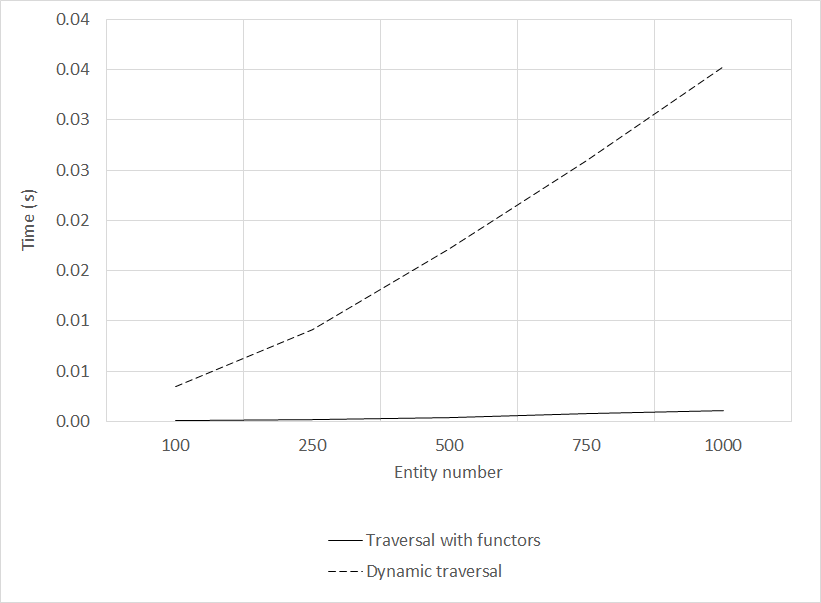
\includegraphics[width=\textwidth]{Figures/chapter_networking/chart}
  \caption{Execution time of Casanova implemented with functors vs the dynamic implementation}
  \label{fig:ch_networking_chart}
\end{figure}

\section{Casanova Networking Primitives with Functors}
\label{sec:ch_networking_functor_networking}
In the previous chapter we described in detail how to implement the logic of the Casanova update traversal with functors in Metacasanova. We also further extended its first implementation with interruptible rules. In this section we show a sketch of how to use functors to implement the networking primitives introduced in Casanova in Section \ref{sec:ch_networking_casanova_networking_primitives}. In what follows we assume that the data transfer primitives are defined in an external library that we assume it is given, since the same applies to the implementation presented in Section \ref{sec:ch_networking_casanova_networking_primitives}, and the send and receive primitives simply generate calls to this library.

\subsection{Network Record}
\label{subsec:ch_networking_network_record}
In order to implement the logic of master/slave entities we need to store additional information in a Casanova entity to know if its instance has been created locally (thus being master). At this purpose we use a functor \texttt{NetworkRecord} to create an instance of a record module to store this information. This functor takes as input a record representing a Casanova entity and builds a new record instance by adding a boolean field used to store the ownership status.

\begin{lstlisting}
Functor "NetworkRecord" => Record : Record 

RecordField "__isLocal" bool r => r'
--------------------------------------
NetworkRecord r => networkRecord
\end{lstlisting}

\subsection{Connection}
\label{subsec:ch_networking_connection}
In order to implement the semantics of a connecting rule we have to modify the field (we rely on the implementation with the record seen in Figure \ref{fig:ch_networking_interruptible_rules}) to store not only the rule continuation but also its connection state. Note that, with this change, we have to change the return type of \texttt{tick} as well, because now the field is a triplet and not a pair. We also define a functor \texttt{ConnectingCoroutine} that instantiate a field updater sharing the same implementation that we generate from a normal coroutine, except for the logic of the function \texttt{update}. 

\begin{lstlisting}
Functor "ConnectingCoroutine" => string => Record => Record => string => stmt : FieldUpdater
\end{lstlisting}

\noindent
This time \texttt{update} has three evaluation rules. The first one creates a getter to retrieve the current field. It then calls the getter generated at the previous step to read the value of the connection status stored in the field. The following clause performs a check on the connection status. If the value is true then the clause fails and thus the rest of the premises is not executed because the whole evaluation rule fails and we skip to the next evaluation rule. If the value is false then we run the code of the rule. At this point if the continuation after the rule update is empty then the connecting rule has terminated its execution and we set to \texttt{true} the connection status. 

\begin{lstlisting}
----------------------------------
ConnectingCoroutine ruleName continuation r field stmts => FieldUpdater r field {
  ...
  
  
  GetField r field => getter
  GetField continuation ruleName => contGetter
  getter.get entity -> (v,(connected,cont))
  connected = false
  tick entity k dt -> (v',(c',k'))
  contGetter.get k' -> nop
  --------------------------
  update entity dt -> (v',(true,k'))
  
  ...
}
\end{lstlisting}

\noindent
The second evaluation rule differs from the first only in the fact that it is executed when the Casanova rule returns a non-empty continuation. In this case we do not set the connection status to \texttt{true} because the connecting rule has not terminated its execution yet.

\begin{lstlisting}
----------------------------------
ConnectingCoroutine ruleName continuation r field stmts => FieldUpdater r field {
  ...
  
  
  GetField r field => getter
  GetField continuation ruleName => contGetter
  getter.get entity -> (v,(connected,cont))
  connected = false
  tick entity k dt -> (v',(c',k'))
  --------------------------
  update entity dt -> (v',(c',k'))
  
  ...
}
\end{lstlisting}

\noindent
The third and final case of the evaluation rule is when the connection status has already been set to \texttt{true}; this means that the Casanova rule has already been evaluated completely during a previous update and does not need to be executed again.\\

\begin{lstlisting}
----------------------------------
ConnectingCoroutine ruleName continuation r field stmts => FieldUpdater r field {
  ...
  

  GetField r field => getter
  getter.get entity -> (v,(connected,continuation))
  connected = true
  getter.get entity -> (v,k)
  ------------------------
  update entity dt -> (v,k)
  
  ...

} 
\end{lstlisting}

\noindent
In the case of a connected rule, we need to be able to detect a new connection. This can be done in different ways: one possible solution is that when a client sends its data during the \texttt{connecting} phase, it sends also information about the connection. This step is handled at low level by the connection primitives. A Casanova rule marked as \texttt{connected} starts with a \texttt{wait} statement that checks if a new client has connected to the system. For the remaining part the rule behaves like a normal coroutine. Of course when the rule body has been completely evaluated, then it stops again until a new client connects, since the whole body will be reconstructed and thus also the \texttt{wait} statement

\subsection{Local and Remote Entities}
\label{subsec:ch_networking_local_and_remote}
The behaviour of master and slave rules can be modelled through dedicated functors that generate different instances for the field updater, in the same fashion as the \texttt{connecting} rule. We thus define two new functors \texttt{MasterCoroutine} and \texttt{SlaveCoroutine}. \texttt{MasterCoroutine} generates a field updater that has two different evaluation rules for \texttt{update}. The first one builds a getter for the field \texttt{\tu\tu isLocal}. It then uses it to read its value from the current entity and uses a clause to check whether the entity is local. At this point, if the entity is not local, the whole evaluation rule fails and the next one is run. Otherwise the Casanova rule body is run and the field updated accordingly to its specific code.

\begin{lstlisting}
Functor "MasterCoroutine" => string => Record => Record => string => stmt : FieldUpdater

----------------------------------------
 MasterCoroutine ruleName continuation r field stmts => FieldUpdater r field {
   ...
   
   GetField r "__isLocal" => localGetter
   localGetter.get entity -> (isLocal,(c,k))
   isLocal = true
   tick entity k dt -> (v',(c',k'))
   ------------------------------
   update entity dt -> (v',(c',k'))
   
   ...
\end{lstlisting}

\noindent
The second evaluation rule is used when the entity is not local. In this case the semantics of a \texttt{master} rule is simply not to be executed. In order to emulate this behaviour we simply return the content of the field as it is (including all the information on the Casanova rule state).
\begin{lstlisting}
----------------------------------------
 MasterCoroutine ruleName continuation r field stmts => FieldUpdater r field {
   ...
   
   GetField r "__isLocal" => localGetter
   GetField r field => getter
   localGetter.get entity -> (isLocal,(c,k))
   isLocal = false
   getter.get entity -> (v,(c,k))
   ------------------------------
   update entity dt -> (v,(c,k))
   
   ...
 }
\end{lstlisting}

\noindent
The \texttt{SlaveCoroutine} functor behaves in an analogous way: it generates two evaluation rules for \texttt{update} that are complementary to those of the \texttt{MasterCoroutine}. In this case the Casanova rule is updated only if the field \texttt{\tu\tu isLocal} is false. If this is not the case the second evaluation rule is triggered and it returns simply the field as it is.

\begin{lstlisting}
----------------------------------------
 SlaveCoroutine ruleName continuation r field stmts => FieldUpdater r field {
   ...

   GetField r "__isLocal" => localGetter
   localGetter.get entity -> (isLocal,(c,k))
   isLocal = false
   tick entity k dt -> (v',(c',k'))
   ------------------------------
   update entity dt -> (v',(c',k'))

   GetField r "__isLocal" => localGetter
   GetField r field => getter
   localGetter.get entity -> (isLocal,(c,k))
   isLocal = true
   getter.get entity -> (v,(c,k))
   ------------------------------
   update entity dt -> (v,(c,k))
   
   ... 
 }
\end{lstlisting}

\noindent
As a final note we want to point out that, since now the semantics of Casanova is encapsulated into the \texttt{FieldUpdater} instance generated by the \texttt{Coroutine} functor, by introducing different kinds of functors able to build the field updaters for coroutines we would need to duplicate the code of the semantics in the field updater modules instantiated by each functor. This is, of course, not a good a practice and the issue can be circumvented by creating an additional module, which we can call \texttt{CasanovaSemantics}, that contains the semantics of all the statements of Casanova. This module is instantiated in each field updater for coroutines by an utility functor defined internally to each field updater. When we need to refer to the semantics of a specific Casanova statement we simply call this functor to generate an instance of the module containing it and then we use it to access the particular evaluation rule that we require for the statement.

\section{Summary}
In this chapter we have presented an extension for the domain-specific language for game development Casanova that introduces abstractions to define the synchronization mechanisms for a multiplayer online game. We then showed a re-implementation of Casanova with functors in Metacasanova and evaluated its performance. The evaluation shows that this new implementation has a running time roughly 42 times faster than the implementation of Casanova shown in Chapter \ref{ch:languages}. We have also shown that functors are flexible enough to implement completely the mechanism of interruptible rules of Casanova and also to implement the same networking abstractions presented for the hard-coded version of the Casanova compiler, of which we provided a sketch. In the next chapter we conclude this dissertation by answering the research questions proposed in Chapter \ref{ch:introduction} and we draw our conclusions.
